% Appendix A

\chapter{Appendices}

\section{A. Further detail of experiments}

\section{Bayesian Inference}

Prior probabilities were calculated or each half-hourly period in a week. Fig \ref{fig10b} shows the calculations for the first 2.5 hours of a Sunday (d-hour-hh format). 

Our parameter of interest is the mean for the Beta distribution representing the probability of play in that time period. We estimate this by calculating probability of a play (total plays in period / count of plays and non-plays) per user, then taking the mean and variance across users. $a$ and $b$ are then determined as:
$a = (\frac{(1- \mu)}{\sigma} - \frac{1}{\mu}) \mu^2$
and
$\beta=\alpha\left(\frac{1}{\mu}-1\right)$.

\begin{figure}[h!]
	\centering
	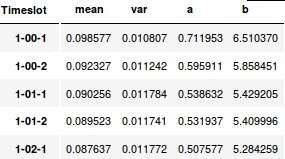
\includegraphics[width=4cm, keepaspectratio,]{fig010b.jpg}
	\caption{}
	\label{fig10b}
\end{figure} 

This allows us to visualize the prior probability for any given time period as shown in \ref{fig10c}.

\begin{figure}[h!]
	\centering
	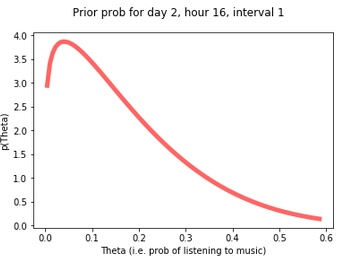
\includegraphics[width=5cm, keepaspectratio,]{fig010c.jpg}
	\caption{}
	\label{fig10c}
\end{figure} 

Once established we can calculate the liklihood of an individual user listening to music in a given time period by passing their observations as they come in for a specific timeslot $s$: $(H_{t,s})$ , into a Beta-Binomial formula to determine the probability of listening at the next occurence of that time slot as shown in <TBC>

Finally the threshold at which we determine that a probability constitutes a Play event is determined by comparing the false positive rates with the true positive rates using a ROC curve (\ref{fig10d}). This tells us that 0.4 is the optimal threshold at which to determine a Play event.

\begin{figure}[h!]
	\centering
	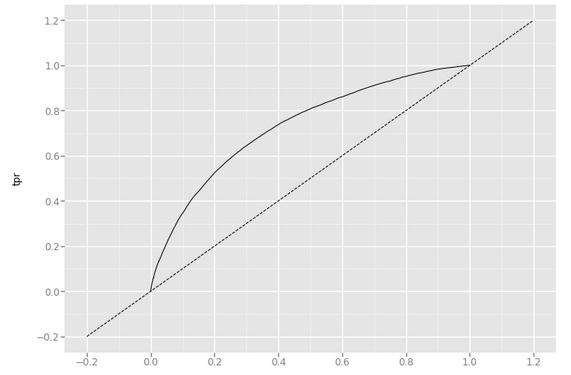
\includegraphics[width=5cm, keepaspectratio,]{fig010d.jpg}
	\caption{ROC curve showing 0.4 as the optimal threshold}
	\label{fig10d}
\end{figure} 

The results from the model are shown in figure \ref{fig10e}. We see that the recall and precision of play events (as denoted by 1) is very low suggesting that relying on a Bayesian approach centered around a weekly profile of each users habits is not an effective method for predicting a play event for a new time period.

\begin{figure}[h!]
	\centering
	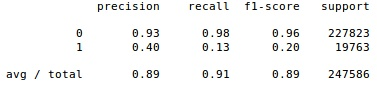
\includegraphics[width=7cm, keepaspectratio,]{fig010e.jpg}
	\caption{Beta-Bionmial Model Results}
	\label{fig10e}
\end{figure} 


\section{Content not used} % Main appendix title

Intro:
While the modeling of aggregate patterns is well understood, these models ofen breakdown when applied to customizing results for individual users. At this level the temporal patterns of an individual combined with the behaviour of the population may be a better predictor of event timing. For instance, sticking with the example above, the times at which a person has lunch during the day may help predict that they will finish work a little later.

